
\chapter{Getting started with PETSc}
\label{chap:getstarted}

\section{A code that does almost nothing, but in parallel}

The purpose of the \PETSc library is to help you solve scientific and engineering problems, such as PDEs of course, on distributed computers.  But \PETSc is built ``on top of'' the Message Passing Interface (MPI; \citep{Groppetal1999}) library, and some of the flavor of that library comes through.  We start with an example C code that is essentially an introductory MPI example, though it calls \PETSc for some basic tasks.

This code \texttt{c1e.c}, shown in its entirety in Figure \ref{code:e}, computes Euler's constant
\begin{equation}
e = \sum_{n = 0}^\infty \frac{1}{n!} \approx 2.718281828 \label{introeseries}
\end{equation}
It does the computation in a distributed manner by computing one term of the infinite series on each process.  Thus it computes a better estimate of $e$ when run on more MPI processes. While this is a silly use of \PETSc, it is an easy to understand parallel computation.

As with any C source for an executable, \texttt{c1e.c} has a function called \texttt{main()} which takes inputs from the command line, namely \texttt{argc} and \texttt{argv},\sidenote{Here \texttt{argc} is an \texttt{int} holding the argument count.  The second argument \texttt{argv} is an array of strings (i.e.~C type \texttt{char**}) holding the command line (i.e.~command and arguments).  However, in all codes in this book we simply pass these arguments on to \PETSc through the \texttt{PetscInitialize()} method.} and which outputs an \texttt{int} which is $0$ if the program succeeds.  Also, like all C codes, we include the needed headers; only \texttt{petscsys.h} is needed here, but later codes will include other \PETSc headers.

The substance of \texttt{main()} is to declare some variables, do a computation on each process, and communicate the results between processes to get an estimate of $e$.  Finally we report success (i.e.~return $0$) at the end.

More details of \texttt{c1e.c} can be described once we compile and run the code.  Please do the following to start:
\begin{cline}
$ cd p4pdes/c/  # download this book, and its codes in p4pdes/c/, by
                #     "git clone https://github.com/bueler/p4pdes.git"
$ make c1e
\end{cline}
For the command ``\texttt{make}'' to work there must be a makefile, of course, and it is \texttt{/p4pdes/c/makefile}, shown in Figure \ref{code:c1emakefile}.  For all the codes in this book, the makefile will have this form, exactly as recommended in the \PETSc User's Manual \citep{petsc-user-ref}.

\inputwhole{../c/c1e.c}{\texttt{p4pdes/c/c1e.c}}{Compute $e$ in parallel.}{code:e}

Run the code on one MPI process like this:
\begin{cline}
$ ./c1e
e is about 1.000000000000000
rank 0 did 1 flops
\end{cline}
%$
The value $1.0$ is a very poor estimate of $e$, but this code does better with more processes:
\begin{cline}
$ mpiexec -n 5 ./c1e
rank 3 did 7 flops
rank 4 did 9 flops
e is about 2.708333333333333
rank 0 did 1 flops
rank 1 did 3 flops
rank 2 did 5 flops
\end{cline}
%$
That's a better estimate of $e$, but hardly impressive.  On the other hand, with $N=20$ processes, and thus $N=20$ terms in series \eqref{introeseries}, we get a good estimate:
\begin{cline}
$ mpiexec -n 20 ./c1e
rank 9 did 19 flops
...
e is about 2.718281828459045
rank 0 did 1 flops
...
rank 18 did 37 flops
\end{cline}
%$

\cinputraw{c1emakefile.frag}{extract from \texttt{p4pdes/c/makefile}}{All \texttt{makefile}s for the \PETSc codes in this book look like this.}{}{//START}{//STOP}{code:c1emakefile}

Now, perhaps the reader is worried that this book was written using a large supercomputer whereas the reader has a little laptop with only a couple of cores.  Not so; these $N=5$ and $N=20$ process MPI calls work just fine on the author's four-core laptop because MPI processes are created as needed.\sidenote{Multitasking operating systems have been around for quite some time!}

The main job in \texttt{c1e.c} is to collect the sum of the terms of (truncated) infinite series \eqref{introeseries} onto each process.  After each process computes term $1/n!$, where $n$ is its rank in the MPI communicator, a call to \texttt{MPI\_Allreduce()} does the sum and then sends the sum back to each process.  We also get the rank of the current process with a call to \texttt{MPI\_Comm\_rank()}.  These direct uses of the MPI library illustrate that \PETSc, which tries to avoid duplication of MPI functionality, need not be called for some low-level parallel tasks.

In \texttt{c1e.c} we print the computed estimate of $e$, and we also have each process print its rank and the work it did.  Observe that \texttt{PetscPrintf()}, a formatted print command like \texttt{fprintf()} from the C standard library, is called twice, once with MPI communicator \texttt{PETSC\_COMM\_WORLD} and once with \texttt{PETSC\_COMM\_SELF}.\sidenote{Thereby we illustrate collective and non-collective operations in the same program.}  The first of these \texttt{STDOUT} printing jobs is therefore \emph{collective} over all processes, and thus only done once, and other printing job is individual to each rank.\sidenote{A process is often just called a \emph{rank} in MPI language.}  In the output the \texttt{PETSC\_COMM\_SELF} printed lines appear in almost random order because the print occurs as soon as that process reaches that line.

Every \PETSc program should start and end with the commands \texttt{PetscInitialize()} and \texttt{PetscFinalize()}:
\begin{code}
PetscInitialize(&argc,&args,(char*)0,help);
... everything else goes here ...
PetscFinalize();
\end{code}
Also, so that this \PETSc code can provide useful usage help, we add a \texttt{help} string at the start; it is a good place to say what the purpose of the code is.

There is one more observation about \texttt{c1e.c} and all \PETSc programs: there is error-checking clutter from capturing and checking the return code of each method called.  While languages other than C could help with decluttering this stuff, we are stuck with lines that look like
\begin{code}
ierr = PetscCommand(...); CHKERRQ(ierr);
\end{code}
The explanation of this clutter is that almost all \PETSc methods, and most user-written methods in \PETSc programs, return an \texttt{int} for error checking, with value $0$ if successful.  In the line above, \texttt{ierr} is a \texttt{PetscInt} type and \texttt{CHKERRQ()} is a macro which does nothing if \texttt{ierr == 0} but which stops the program otherwise.  In the nonzero case the program stops with a traceback, namely a list of the nested methods, in reverse order, showing the line numbers and method names of the location where the error occurred.  This traceback tends to be the first line of defense when debugging run-time errors.  Examples in this book always capture-and-check the returned error code in this way, despite the clutter.  On the other hand, after this chapter we will strip the ``\texttt{ierr =}'' and ``\texttt{CHKERRQ(ierr);}'' clutter from the code displayed in the text, even though it is still present in the source file itself.


\section{Linear systems}

Of course, our goal in the remainder of the book is to compute more interesting quantities than Euler's constant $e$.  At the core of most \PETSc computations is a finite-dimensional linear system.  Before solving such systems in \PETSc, it is useful to recall the most basic ideas of numerical linear algebra.

Suppose $\bb\in \RR^{N}$ is a column vector and $A\in\RR^{N\times N}$ is a square matrix.  The linear system
\begin{equation}
A \bu = \bb \label{introsystem}
\end{equation}
has a unique solution if $A$ is invertible, namely
\begin{equation}
\bu = A^{-1} \bb. \label{introsolution}
\end{equation}
This is simple in theory.

It is not so simple in practice, however, when solving large systems on a computer.  There are two key facts to keep in mind while working numerically  \citep{TrefethenBau}.
\renewcommand{\labelenumi}{\roman{enumi})}
\begin{enumerate}
\item \emph{limit to accuracy}:  If real numbers are represented on the computer with machine precision $\eps$ then the solution of \eqref{introsystem} can only be computed within an error $\kappa(A) \eps$ where $\kappa(A) = \|A\|_2 \|A^{-1}\|_2$ is the (2-norm) \emph{condition number} of $A$.\sidenote{Fact i) is about \emph{conditioning} not \emph{methods}.  Informally speaking, there are linear systems $A,\bb$ that are the same to within $\eps$ but for which the infinite-precision solutions $\bu$ are different by the amount $\kappa(A) \eps$.}
\item \emph{cost of direct solutions}:  Computation of solution \eqref{introsolution} by a direct method like Gauss elimination, whether actually forming $A^{-1}$ or not, is an $O(N^3)$ operation.
\end{enumerate}

For a sense of the consequences of these facts, let's put in some numbers for $\eps$, $\kappa(A)$, and $N$.  On most computers the precision for the C \texttt{double} type, the modern default 64-bit representation of real numbers, is $\eps = 2.2 \times 10^{-16}$.  By i), a linear system having $\kappa(A) \approx 10^{10}$, for example, can only be solved to about six digits of precision.

Regarding computational cost, because of ii) a linear system with $N=10^6$ equations requires $\sim 10^{18}$ operations to solve by Gauss elimination.  While even modern supercomputers take a while to do a quintillion operations, so that Gauss elimination is impractical for systems of $N=10^6$ equations, we will successfully solve problems of this size on a single processor in a few seconds, and in $O(N)$ operations, in Chapter \ref{chap:multigrid}.
%time ./c4poisson -da_refine 7 -ksp_type cg -pc_type mg
%on 1153 x 1153 grid:  iterations 2, residual norm = 1.88082e-05
%real 11.18

To build our first \PETSc code for a linear system, we describe the \PETSc objects which store vectors and matrices.


\section{\PETSc \pVec and \pMat objects}

The \pVec object is a container and interface for a distributed vector, and a \pMat object holds a distributed matrix.  Although \PETSc is written in C, not C++, it is a relentlessly object-oriented software library.  Consider the operations which might touch a matrix object \texttt{A} in a linear system like \eqref{introsystem}:
\begin{code}
Mat A;
MatCreate(COMM,&A);
MatSetSizes(A,PETSC_DECIDE,PETSC_DECIDE,N,N);
PetscObjectSetName((PetscObject)A,"A");
MatSetOptionsPrefix(A,"a_");
MatSetFromOptions(A);
... fill entries of (i.e. assemble) A ...
... solve system with A ...
MatDestroy(&A);
\end{code}
In fact, for ``\pVec'' objects storing vectors, ``\pMat'' objects storing matrices, and indeed for all \PETSc object types, this basic sequence of operations applies:
\begin{code}
Object X;
ObjectCreate(COMM,&X);
... set properties of X from code ...
ObjectSetFromOptions(X);  // allows run-time setting of properties
... use X ...
ObjectDestroy(&X);
\end{code}
Of course ``\texttt{Object}'' here is merely a meta-name for a \PETSc type like \pVec or \pMat.

\PETSc objects are generically distributed across, and accessible from, multiple MPI processes.  Therefore the first argument of an \texttt{ObjectCreate()} method is an MPI communicator (``\texttt{COMM}'').  All processes in \texttt{COMM} must call the \texttt{ObjectCreate()} method.

Evidently \texttt{Mat A} above has an internal representation with nontrivial structure, but that is hidden.  Indeed the data structure inside \texttt{A} depends on runtime choices, the most basic being that the number of bytes used to store \texttt{A} on a given MPI process will depend on the number of processes.  At a deeper level, a \PETSc \pMat object need not even \emph{have} entries, but it may instead represent code that applies a linear operator to vectors.

Because of the call to \texttt{MatSetOptionsPrefix()}, run-time options can specifically address the particular \pMat object.  For example, the run-time option \texttt{-a\_mat\_view} will print out the entries of \texttt{A}.  An option prefix like ``\texttt{a\_}'' is especially helpful in distinguishing \pMat objects at the command line in a context with multiple \pMats.

Once \texttt{A} is created and set up by the first five commands \texttt{MatCreate()}--\texttt{MatSetFromOptions()}, then various methods become valid for \texttt{A}, for example including the \texttt{MatSetValues()} method to set entries in \texttt{A}.


\section{Assembly and parallel layout of \pVecs and \pMats}

Fundamentally, a \pVec or \pMat can store its entries in parallel across all the processes in the MPI communicator used when creating it.  For the \pVec type, the create-assemble sequence of a vector with four entries might look like
\begin{code}
Vec x;
PetscInt   i[4] = {0, 1, 2, 3};
PetscReal  vals[4] = {11.0, 7.0, 5.0, 3.0};

VecCreate(COMM,&x);
VecSetSizes(x,PETSC_DECIDE,4);
VecSetFromOptions(x);
VecSetValues(x,4,i,vals,INSERT_VALUES);
VecAssemblyBegin(x);
VecAssemblyEnd(x);
\end{code}
The four entries of \texttt{Vec x} are (obviously) set by \texttt{VecSetValues()}, putting values from array \texttt{vals[]} at the indices given by \texttt{i[]}.  Potentially such operations require communication between processes, because entries of \texttt{x} which are stored on process $m$ could be set by processor $n$.  Such communication is started and ended by the \texttt{VecAssemblyBegin(), VecAssemblyEnd()} pair of commands.

\begin{marginfigure}
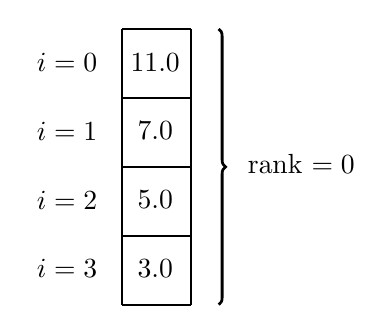
\begin{tikzpicture}[scale=3.5]
  \pgfmathsetmacro\fourth{1.0/4.0}
  \pgfmathsetmacro\xoff{0.12}
  \pgfmathsetmacro\yoff{0.12}
  \draw[xstep=\fourth,ystep=\fourth,black,thick] (0.0,0.0) grid (\fourth,1.0);
  \node at (-0.2,1.0-\yoff) {$i=0$};
  \node at (\xoff,1.0-\yoff) {$11.0$};
  \node at (-0.2,0.75-\yoff) {$i=1$};
  \node at (\xoff,0.75-\yoff) {$7.0$};
  \node at (-0.2,0.5-\yoff) {$i=2$};
  \node at (\xoff,0.5-\yoff) {$5.0$};
  \node at (-0.2,0.25-\yoff) {$i=3$};
  \node at (\xoff,0.25-\yoff) {$3.0$};
  \draw[decoration={brace,mirror,raise=5pt},decorate,line width=1pt] (0.3,0.0) -- (0.3,1.0);
  \node at (0.65,0.51) {rank $=0$};
\end{tikzpicture}
\bigskip
\caption{A sequential \pVec layout, all on rank $=0$ process.}
\label{fig:seqveclayout}
\end{marginfigure}

Suppose this sequence appears in a program called \texttt{myprogram.c}.  If the program is run sequentially on one process, i.e.~as
\begin{cline}
$ ./myprogram.c
\end{cline}
%$
then, at the end of the above create-assemble sequence, the storage of \texttt{x} looks like Figure \ref{fig:seqveclayout}.

However, if run as
\begin{cline}
$ mpiexec -n 2 ./myprogram.c
\end{cline}
%$
then the layout looks like Figure \ref{fig:mpitwoveclayout}.  In this case the argument \texttt{PETSC\_DECIDE} in \texttt{VecSetSizes()} is active because \PETSc \emph{decides} to put the first two entries of \texttt{x} on the rank $0$ process and the other two on the rank $1$ process. 

\begin{marginfigure}
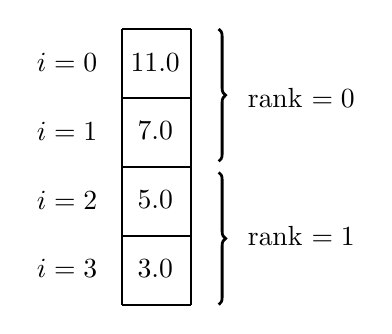
\begin{tikzpicture}[scale=3.5]
  \pgfmathsetmacro\fourth{1.0/4.0}
  \pgfmathsetmacro\xoff{0.12}
  \pgfmathsetmacro\yoff{0.12}
  \draw[xstep=\fourth,ystep=\fourth,black,thick] (0.0,0.0) grid (\fourth,1.0);
  \node at (-0.2,1.0-\yoff) {$i=0$};
  \node at (\xoff,1.0-\yoff) {$11.0$};
  \node at (-0.2,0.75-\yoff) {$i=1$};
  \node at (\xoff,0.75-\yoff) {$7.0$};
  \node at (-0.2,0.5-\yoff) {$i=2$};
  \node at (\xoff,0.5-\yoff) {$5.0$};
  \node at (-0.2,0.25-\yoff) {$i=3$};
  \node at (\xoff,0.25-\yoff) {$3.0$};
  \draw[decoration={brace,mirror,raise=5pt},decorate,line width=1pt] (0.3,0.52) -- (0.3,1.0);
  \node at (0.65,0.752) {rank $=0$};
  \draw[decoration={brace,mirror,raise=5pt},decorate,line width=1pt] (0.3,0.0) -- (0.3,0.48);
  \node at (0.65,0.251) {rank $=1$};
\end{tikzpicture}
\bigskip
\caption{A parallel \pVec layout on two processes.  Because we call ``\texttt{VecSetSizes(x,PETSC\_DECIDE,4)}'', \PETSc decides to split the storage in the middle.}
\label{fig:mpitwoveclayout}
\end{marginfigure}

Though in the current context it is completely artificial, one could override the ``\texttt{PETSC\_DECIDE}'' parallel layout by replacing the \texttt{VecSetSizes()} line with this block of code:
\begin{code}
PetscMPIInt rank;
MPI_Comm_rank(COMM,&rank);
if (rank == 0) {
  VecSetSizes(x,3,4);
} else if (rank == 1) {
  VecSetSizes(x,1,4);
} else {
  SETERRQ(COMM,1,"this code only works with size==2 communicators");
}
\end{code}
That is, we could specify the ``local size'' argument to \texttt{VecSetSizes()}, instead of using \texttt{PETSC\_DECIDE}.\sidenote{In fact such inflexible coding is rarely necessary.}  The resulting layout is shown in Figure \ref{fig:artificialmpitwoveclayout}.

In summary, the reader is allowed to think of a \PETSc \pVec as a one-dimensional C array with its range of indices and contents ``broken-up'' across the processes in the MPI communicator used in the \texttt{VecCreate()} command.

Parallel matrix objects \pMat, which are at some level conceived as 2D arrays, obviously require an additional choice regarding distribution.  But \PETSc makes this choice inside the implementation of \pMat.  Namely, \PETSc always stores ranges of complete rows on each process.  Said another way, conceptually at least, the column vectors which form the \pMat are stored like \pVecs.

While other storage formats are possible, the one usually used in this book is \emph{parallel compressed sparse row storage}, what \PETSc calls the \texttt{MATMPIAIJ} type.  That is, a range of rows is owned by each process (parallel row storage), and within each owned range of rows only the nonzero entries are stored (sparse), and furthermore the data structures store these nonzero entries contiguously in an array, with an additional contiguous index array (compressed).

\begin{marginfigure}
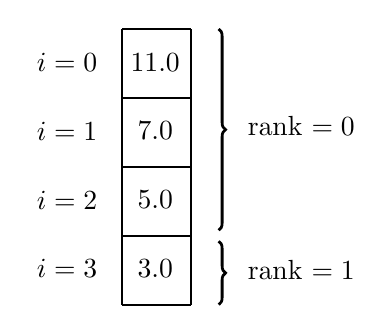
\begin{tikzpicture}[scale=3.5]
  \pgfmathsetmacro\fourth{1.0/4.0}
  \pgfmathsetmacro\xoff{0.12}
  \pgfmathsetmacro\yoff{0.12}
  \draw[xstep=\fourth,ystep=\fourth,black,thick] (0.0,0.0) grid (\fourth,1.0);
  \node at (-0.2,1.0-\yoff) {$i=0$};
  \node at (\xoff,1.0-\yoff) {$11.0$};
  \node at (-0.2,0.75-\yoff) {$i=1$};
  \node at (\xoff,0.75-\yoff) {$7.0$};
  \node at (-0.2,0.5-\yoff) {$i=2$};
  \node at (\xoff,0.5-\yoff) {$5.0$};
  \node at (-0.2,0.25-\yoff) {$i=3$};
  \node at (\xoff,0.25-\yoff) {$3.0$};
  \draw[decoration={brace,mirror,raise=5pt},decorate,line width=1pt] (0.3,0.27) -- (0.3,1.0);
  \node at (0.65,0.65) {rank $=0$};
  \draw[decoration={brace,mirror,raise=5pt},decorate,line width=1pt] (0.3,0.0) -- (0.3,0.23);
  \node at (0.65,0.125) {rank $=1$};
\end{tikzpicture}
\bigskip
\caption{A non-default parallel \pVec layout on two processes, by forcing local sizes to be not equal.}
\label{fig:artificialmpitwoveclayout}
\end{marginfigure}

For example, the following code creates and assembles a \pMat \texttt{A} with four rows and four columns:
% see testmatcreate.c
\begin{code}
Mat A;
PetscInt  i, j[3];
PetscReal v[3];

MatCreate(PETSC_COMM_WORLD,&A);
MatSetSizes(A,PETSC_DECIDE,PETSC_DECIDE,4,4);
MatSetFromOptions(A);
MatSetUp(A);

i = 0;
j[0] = 0;    j[1] = 1;
v[0] = 4.0;  v[1] = -1.0;
MatSetValues(A,1,&i,2,j,v,INSERT_VALUES);
i = 1;
j[0] = 0;    j[1] = 1;    j[2] = 2;
v[0] = -1.0; v[1] = 4.0;  v[2] = -1.0;
MatSetValues(A,1,&i,3,j,v,INSERT_VALUES);
i = 2;
j[0] = 1;    j[1] = 2;    j[2] = 3;
MatSetValues(A,1,&i,3,j,v,INSERT_VALUES);
i = 3;
j[0] = 2;    j[1] = 3;
MatSetValues(A,1,&i,2,j,v,INSERT_VALUES);

MatAssemblyBegin(A,MAT_FINAL_ASSEMBLY);
MatAssemblyEnd(A,MAT_FINAL_ASSEMBLY);
\end{code}
The method \texttt{MatSetValues()} sets a \emph{block} of values, and in this case we use it to set each row of the matrix.  Thus ``\texttt{1,\&i}'' arguments to \texttt{MatSetValues()} say ``we are setting one row, and look at the location of integer \texttt{i} for the (global) index.''  The ``\texttt{3,\&j}'' arguments, used in the \texttt{i} $=1,2$ rows, say ``we are setting three values in the row, and look at integer array \texttt{j} for the (global) indices.''

If the above lines appeared in \texttt{myprogram.c}, and if it was run
\begin{cline}
$ mpiexec -n 2 ./myprogram
\end{cline}
%$
then this \pMat would have the entries and layout shown in Figure \ref{fig:mpitwomatlayout}.

\begin{marginfigure}
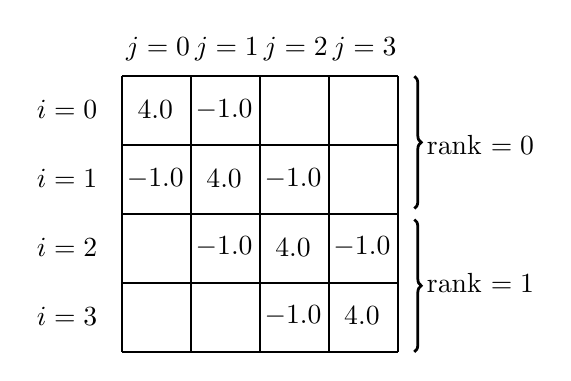
\begin{tikzpicture}[scale=3.5]
  \pgfmathsetmacro\fourth{1.0/4.0}
  \pgfmathsetmacro\xoff{0.12}
  \pgfmathsetmacro\yoff{0.12}
  \draw[xstep=\fourth,ystep=\fourth,black,thick] (0.0,0.0) grid (1.0,1.0);

  \node at (-0.2, 1.0-\yoff) {$i=0$};
  \node at (-0.2,0.75-\yoff) {$i=1$};
  \node at (-0.2, 0.5-\yoff) {$i=2$};
  \node at (-0.2,0.25-\yoff) {$i=3$};

  \node at ( 1.0-\xoff, 1.1) {$j=3$};
  \node at (0.75-\xoff, 1.1) {$j=2$};
  \node at ( 0.5-\xoff, 1.1) {$j=1$};
  \node at (0.25-\xoff, 1.1) {$j=0$};

  \node at (\xoff,1.0-\yoff) {$4.0$};
  \node at (0.25+\xoff,1.0-\yoff) {$-1.0$};

  \node at (\xoff,0.75-\yoff) {$-1.0$};
  \node at (0.25+\xoff,0.75-\yoff) {$4.0$};
  \node at (0.5+\xoff,0.75-\yoff) {$-1.0$};

  \node at (0.25+\xoff,0.5-\yoff) {$-1.0$};
  \node at (0.5+\xoff,0.5-\yoff) {$4.0$};
  \node at (0.75+\xoff,0.5-\yoff) {$-1.0$};

  \node at (0.5+\xoff,0.25-\yoff) {$-1.0$};
  \node at (0.75+\xoff,0.25-\yoff) {$4.0$};

  \draw[decoration={brace,mirror,raise=5pt},decorate,line width=1pt] (1.01,0.52) -- (1.01,1.0);
  \node at (1.3,0.752) {rank $=0$};
  \draw[decoration={brace,mirror,raise=5pt},decorate,line width=1pt] (1.01,0.0) -- (1.01,0.48);
  \node at (1.3,0.251) {rank $=1$};
\end{tikzpicture}
\bigskip
\caption{A parallel \pMat layout on two processes.  Blank entries are zeros, which are not stored because of ``compressed sparse'' storage.}
\label{fig:mpitwomatlayout}
\end{marginfigure}

We can have \PETSc show us the \pMat in different formats at the command line:
\begin{cline}
$ ./myprogram -mat_view
Mat Object: 1 MPI processes
  type: seqaij
row 0: (0, 4)  (1, -1)
row 1: (0, -1)  (1, 4)  (2, -1)
row 2: (1, -1)  (2, 4)  (3, -1)
row 3: (2, -1)  (3, 4)
$ ./myprogram -mat_view ::ascii_dense
Mat Object: 1 MPI processes
  type: seqaij
 4.00000e+00  -1.00000e+00  0.00000e+00  0.00000e+00
 -1.00000e+00  4.00000e+00  -1.00000e+00  0.00000e+00
 0.00000e+00  -1.00000e+00  4.00000e+00  -1.00000e+00
 0.00000e+00  0.00000e+00  -1.00000e+00  4.00000e+00
\end{cline}
The former view shows the compressed sparse storage, wherein only the nonzero values are shown, as pairs with column index and value, while the latter is a traditional (``dense'') display where zero values are shown.  In these cases the matrix was stored in \emph{serial} compressed sparse row format, the \texttt{MATSEQAIJ} type.

The result vector of a \pMat-\pVec product is, of course, a linear combination of the columns of the \pMat.  Thus, in practice, ``parallel row storage'' layout normally means two things:\begin{itemize}
\item \PETSc internally distributes the rows of the \pMat $A$ the same way as the entries of the intended output \pVec $b$, i.e.~if $Ax=b$ for some $x$, at least when \texttt{PETSC\_DECIDE} is used in setting the \pMat sizes, and
\item before \PETSc multiplies a matrix times a vector, \PETSc automatically communicates (``scatters'') the whole vector to each process.
\end{itemize}
After the scatter the \pMat-\pVec product is a local operation, requiring no further communication.

FIXME: assembly of \pMat a bit idiosyncratic; \texttt{MatSetValues()} sets a \emph{block} of values, not arbitrary inserts into sparse storage; need either MatXXXSetPreallocation() or MatSetUp() before MatGetOwnershipRange()


\section{Solve a linear system in \PETSc}

\cinputpartnostrip{c1matvec.c}{Initialize \PETSc and set up \pVecs and \pMat.}{I}{}{//ENDSETUP}{code:matvecpartone}

FIXME: emphasize that \texttt{MatGetOwnershipRange()} means that different processes are assembling different rows, unlike earlier example where all processes inserted all values

\cinputpartnostrip{c1matvec.c}{Assemble \pMat $A$.  Assemble right-hand side $b$ via exact solution to system.}{II}{//ENDSETUP}{//ENDASSEMBLY}{code:matvecparttwo}

\cinputpartnostrip{c1matvec.c}{Set up \pKSP.  Solve.  Finalize.}{III}{//ENDASSEMBLY}{//END}{code:matvecpartthree}

FIXME: show sparse and Matlab-format output for \texttt{A}, noting we get this at the \texttt{MatAssemblyEnd()} stage %$ ./c1matvec -a_mat_view ::ascii_matlab

FIXME: solve without choosing method

FIXME: show how to solve with Gaussian elimination


\section{A bit more numerical linear algebra}

Many methods other than Gauss elimination are possible for solving linear systems.  Usually these methods are iterative, and they often use the \emph{residual}.  By definition, if $\bu_0\in \RR^N$ is a vector then by the residual for $\bu_0$, as an estimate of the solution to equation \eqref{introsystem}, is the vector
\begin{equation}
\br_0 = \bb - A \bu_0. \label{residualdefn}
\end{equation}

Evaluating the residual for a known vector $\bu_0$ requires only applying $A$ to it, an $O(N^2)$ operation at most.  However, most discretization schemes for PDEs generate matrices $A$ that are \emph{sparse}, with many more zero entries than nonzeros, and often the number of nonzeros per row is independent of $N$.  In such cases the operation $A\bu_0$ can be implemented in $O(N)$ operations.

The \emph{Richardson iteration} is an example of an iterative method based on the residual.  If $\bu_0$ is an initial estimate of the solution then it simply adds a multiple $\omega$ of the residual at each step:
\begin{equation}
\bu_{k+1} = \bu_k + \omega (\bb - A \bu_k).  \label{introrichardson}
\end{equation}
If significantly fewer than $O(N^2)$ steps are needed to make $\bu_k$ an adequate approximation of the exact solution $\bu$, then the Richardson iteration can improve on Gauss elimination.  On the other hand, the Richardson iteration may not converge.

\newcommand{\rvect}[3]{\ensuremath{\bu_{#1} = \begin{bmatrix} #2 \\ #3 \end{bmatrix}}}

\medskip\noindent\hrulefill
\begin{example} Consider the linear system
\begin{equation}
A \bu
= \begin{bmatrix}
10 & -1 \\ -1 & 1
\end{bmatrix}
\begin{bmatrix} u_1 \\ u_2 \end{bmatrix}
= \begin{bmatrix} 8 \\ 1 \end{bmatrix}
= \bb
 \label{introexample}
\end{equation}
which has solution $\bu = [1\,\, 2]^\top$.  If we start with estimate $\bu_0 = [0\,\, 0]^\top$ then the unweighted ($\omega=1$) Richardson iteration \eqref{introrichardson} gives a sequence of vectors % see ../matlab/richardsonex.m
\begin{equation}
\rvect{0}{0}{0}, \rvect{1}{8}{1}, \rvect{2}{-63}{9}, \rvect{3}{584}{-62}, \dots
\end{equation}
This sequence is not heading toward the solution $\bu = [1\,\, 2]^\top$.
\end{example}
\noindent\hrulefill

If we rewrite \eqref{introrichardson} as
\begin{equation}
\bu_{k+1} = (I - \omega A) \bu_k + \omega \bb  \label{introrewriterichardson}
\end{equation}
then it is easy to believe that the ``size'' of the matrix $I-\omega A$ will determine whether $\lim_{k\to\infty} \bu_k$ exists, for generic starting vectors $\bu_0$.

To examine such questions, we recall the definitions of \emph{eigenvalue} and \emph{singular value}.  A complex number $\lambda \in \CC$ is an eigenvalue of a square matrix $B\in\RR^{N\times N}$ if there is a nonzero vector $\bv\in\CC^N$ so that $B \bv = \lambda \bv$.    The singular values are the square roots of the eigenvalues of the matrix $B^*B$.\sidenote{The matrix $B^*B$ is symmetric and positive-definite so its eigenvalues are nonnegative.}  Singular values are also geometrically-defined as the lengths of semi-axes of the ellipsoid in $\RR^N$ that results from applying $B$ to all vectors in the unit sphere of $\RR^N$ \citep{TrefethenBau}.

The set of all eigenvalues of $B$ is the \emph{spectrum} $\sigma(B)$ of $B$, and properties of matrices that can be described in terms of eigenvalues or singular values are generically called ``spectral properties.''  For example, recall that $\|B\|_2$ is equal to the largest singular value of $B$, while $\|B^{-1}\|_2$ is equal to the inverse of the smallest singular value of $B$.  The 2-norm condition number $\kappa(B)$ is the ratio of largest to smallest singular values,\sidenote{The condition number of $B$ well-visualized as the eccentricity of the ellipsoid we used in defining the singular values geometrically.}, and thus is a spectral property of $B$.

It is an easy exercise to show that the Richardson iteration \eqref{introrichardson} will converge if and only if all the eigenvalues of $B=I-\omega A$ are inside the unit circle.  Defining the \emph{spectral radius} $\rho(B)$ of a matrix $B$ as the maximum norm of the eigenvalues of $A$, we can describe the convergence of the Richardson iteration this way:
\begin{equation}
\text{\eqref{introrichardson} converges if and only if } \rho(I-\omega A) < 1. \label{introconvergethm}
\end{equation}
We can also show that $\rho(B) \le \|B\|_2$ so \eqref{introrewriterichardson} converges if $\|I-\omega A\|_2 < 1$, but this norm condition is merely sufficient, while \eqref{introconvergethm} is necessary and sufficient.

Other examples of iterative methods include the classical Jacobi and Gauss-Siedel iterations.  The most powerful methods generate optimal, in various senses \citep{TrefethenBau}, estimates $\bu_k$ which are each linear combinations of vectors $\bb,A\bb,A^2\bb,\dots,A^{k-1}\bb$.  These methods are collectively called \emph{Krylov space methods} because the span of these vectors is a Krylov space.  Typically the effectiveness of the iteration on a given matrix $A$ depends on the eigenvalues or singular values of $A$.  We use Krylov space methods in Chapter \ref{chap:structured} and all later Chapters.  Examples are conjugate gradients (CG) and minimum residual methods (e.g.~MINRES or GMRES) \citep{Greenbaum1997}.

There are many other systems which are equivalent to \eqref{introsystem}.  In fact, if $P\in\RR^{N\times N}$ is an invertible square matrix then the systems
\begin{equation}
(P^{-1} A) \bu = P^{-1} \bb \label{introleftpre}
\end{equation}
and
\begin{equation}
(A P^{-1}) (P\bu) = \bb \label{introrightpre}
\end{equation}
obviously have the same solution $\bu$ as \eqref{introsystem}.  However, matrices $P^{-1} A$ or $A P^{-1}$ may have different eigenvalues, condition numbers, and so on, namely different spectral properties, from $A$.  While the accuracy of the approximate solution $\bu$ cannot be improved beyond the $\kappa(A) \eps$ level---fact i) cannot be overcome in that sense---methods can indeed take advantage of better conditioning or other spectral properties to generate $\bu$ more quickly.  Especially if $P^{-1}$ is easy to apply\sidenote{The inverse matrix $P^{-1}$ is ``easy to apply'' exactly if the system $P\bv = \bc$ is easy to solve for $\bv$ in the sense of low computational cost.} then this can be an advantageous idea when trying to approximate $\bu$ quickly.  Equivalent systems \eqref{introleftpre} and \eqref{introrightpre} are referred to as \emph{preconditioned} systems, with \eqref{introleftpre} called \emph{left preconditioning} and \eqref{introrightpre} called \emph{right-preconditioning}.  Preconditioning can help in making our Richardson iteration example converge.  

\medskip\noindent\hrulefill
\begin{examplecont}  Suppose we use the diagonal matrix from  \eqref{introexample} as $P$:
\begin{equation}
P = \begin{bmatrix}
10 & 0 \\ 0 & 1
\end{bmatrix}.  \label{introP}
\end{equation}
Being diagonal, this $P$ is easy to invert and apply.  The preconditioned Richardson iteration using $P$, namely
\begin{equation}
\bu_{k+1} = \bu_k + \omega (P^{-1} \bb - P^{-1} A \bu_k),  \label{introprerichardson}
\end{equation}
is much better behaved.  With $\bu_0 = [0\,\, 0]^*$ again we get this sequence from \eqref{introprerichardson}:
\begin{equation}
\rvect{0}{0}{0}, \rvect{1}{0.8}{1.0}, \rvect{2}{0.9}{1.8}, \rvect{3}{0.98}{1.90}, \dots
\end{equation}
This sequence is apparently going to $\bu = [1\,\, 2]^*$.  Of course, the explanation is not hard to see; in this case
\begin{equation}
\rho(I-A) = -9.1, \qquad \rho(I-P^{-1} A) = 0.32.
\end{equation}
Convergence claim \eqref{introconvergethm} matches this bit of evidence.
\end{examplecont}
\noindent\hrulefill

Many iterative methods superior to the Richardson iteration are implemented in \PETSc.  We will use several of them, with choice of method only at run-time.


\caveat{But \Matlab is all you want if scale does not matter.}


\section{Exercises}

\renewcommand{\labelenumi}{\arabic{chapter}.\arabic{enumi}\quad}
\begin{enumerate}
\item Program \texttt{c1e.c} does a terrible job of load-balancing because the computation of the factorial $n!$ requires more flops when the process rank is larger.  Modify the code to balance the load almost perfectly, with exactly one multiply operation on each \texttt{rank>0} process, by using a blocking send and receive operations (\texttt{MPI\_Send(),MPI\_Recv()}) to pass the result of the last factorial to the next rank.  (\emph{Of course now we have a code that does a ridiculous amount of communication.})
% e1balanced.c
\item Modify \texttt{c1matvec.c} to read an integer option\sidenote{Use methods \texttt{PetscOptionsBegin()}, \texttt{PetscOptionsInt()}, and \texttt{PetscOptionsEnd()} so that \texttt{-help} output explains the option.} \texttt{-N} and form an $N\times N$ matrix, with $-2$ on the diagonal and $1$ on the super- and sub-diagonals as before.  (Choose any desired right-hand-side.)  Use \PETSc runtime options to estimate the condition number of the matrix for sample $N$ values; the online \PETSc FAQ page\sidenote{\texttt{www.mcs.anl.gov/petsc/documentation/faq.html}} will help with these options.
% see "How can I determine the condition number of a matrix?" on the PETSc FAQ page; "be sure to avoid restarts"
% -pc_type none -ksp_type gmres -ksp_monitor_singular_value -ksp_gmres_restart 1000
\end{enumerate}